\documentclass[tikz,border=6pt]{standalone}
\usepackage{tikz}
\usetikzlibrary{arrows.meta,backgrounds,calc,fit,positioning,shapes.geometric,shapes.misc}

\definecolor{macroblue}{HTML}{4C78A8}
\definecolor{midgreen}{HTML}{59A14F}
\definecolor{microorange}{HTML}{F28E2B}
\definecolor{softgray}{HTML}{F4F4F4}
\definecolor{chipgray}{HTML}{E4E6E8}
\definecolor{edgegray}{HTML}{B8BDC3}
\definecolor{textgray}{HTML}{4D4D4D}

\colorlet{hiddenflowcolor}{macroblue!92!black}
\colorlet{featureflowcolor}{microorange!95!black}
\colorlet{metaflowcolor}{black!55}

\tikzset{
  >={Latex[length=2.5mm,width=2.2mm]},
  every node/.style={inner sep=0pt,outer sep=0pt},
  figure label/.style={font=\scriptsize\sffamily\bfseries,text=textgray},
  section label/.style={font=\scriptsize\sffamily,text=textgray},
  band text/.style={font=\scriptsize\sffamily\bfseries,text=black!85,align=center},
  tokenbox/.style={rounded corners=2pt, draw=edgegray, fill=white, line width=0.6pt},
  sourcebox/.style={rounded corners=5pt, draw=edgegray, fill=white, line width=0.6pt},
  panelbox/.style={rounded corners=7pt, draw=black!12, fill=white, line width=0.7pt},
  neutralchip/.style={rounded corners=2pt, draw=edgegray!90, fill=chipgray, line width=0.45pt},
  cuepill/.style={rounded corners=3pt, draw=edgegray!90, fill=softgray, line width=0.5pt},
  legendtext/.style={font=\scriptsize\sffamily,text=textgray},
  stagehead/.style={rounded corners=4pt, line width=0.6pt},
  attnbox/.style={rounded corners=4pt, draw=edgegray!95, fill=softgray, line width=0.6pt},
  simplebox/.style={rounded corners=4pt, draw=edgegray!95, fill=white, line width=0.6pt},
  routerbox/.style={rounded corners=3pt, draw=edgegray!95, fill=softgray, line width=0.55pt},
  expertbox/.style={rounded corners=2pt, draw=edgegray!95, fill=white, line width=0.5pt},
  hiddenflow/.style={->, draw=hiddenflowcolor, line width=1.1pt},
  featureflow/.style={->, draw=featureflowcolor, line width=1.0pt, dash pattern=on 3.2pt off 1.8pt},
  metaflow/.style={->, draw=metaflowcolor, line width=0.55pt},
}

\newcommand{\fmoeTokenNode}[3]{%
  \begin{scope}[shift={({#1},{#2})}]
    \path[tokenbox] (-0.42,-0.34) rectangle (0.42,0.34);
    #3
  \end{scope}%
}

\newcommand{\fmoeBallIcon}{%
  \draw[line width=0.45pt, draw=textgray] (0,0) circle [radius=0.16];
  \draw[line width=0.35pt, draw=textgray] (-0.11,0) -- (0.11,0);
  \draw[line width=0.35pt, draw=textgray] (0,-0.11) -- (0,0.11);
  \draw[line width=0.3pt, draw=textgray] (-0.09,-0.09) -- (0.09,0.09);
  \draw[line width=0.3pt, draw=textgray] (-0.09,0.09) -- (0.09,-0.09);
}

\newcommand{\fmoeBootsIcon}{%
  \filldraw[draw=textgray, fill=black!10, line width=0.35pt]
    (-0.16,-0.03) -- (-0.02,-0.03) -- (0.02,-0.11) -- (-0.15,-0.11) -- cycle;
  \filldraw[draw=textgray, fill=black!10, line width=0.35pt]
    (0.01,0.04) -- (0.16,0.04) -- (0.19,-0.05) -- (0.02,-0.05) -- cycle;
}

\newcommand{\fmoeJerseyIcon}{%
  \filldraw[draw=textgray, fill=black!8, line width=0.35pt]
    (-0.13,0.12) -- (-0.04,0.12) -- (0,0.05) -- (0.04,0.12) -- (0.13,0.12) --
    (0.17,0.02) -- (0.09,-0.03) -- (0.08,-0.16) -- (-0.08,-0.16) -- (-0.09,-0.03) -- (-0.17,0.02) -- cycle;
}

\newcommand{\fmoeGuardIcon}{%
  \filldraw[draw=textgray, fill=black!9, line width=0.35pt]
    (0,0.16) -- (0.12,0.1) -- (0.09,-0.1) -- (0,-0.17) -- (-0.09,-0.1) -- (-0.12,0.1) -- cycle;
}

\newcommand{\fmoeSocksIcon}{%
  \filldraw[draw=textgray, fill=black!8, line width=0.35pt]
    (-0.13,0.14) rectangle (-0.04,-0.02);
  \filldraw[draw=textgray, fill=black!8, line width=0.35pt]
    (-0.04,-0.02) -- (0.03,-0.02) -- (0.03,-0.09) -- (-0.1,-0.09) -- cycle;
  \filldraw[draw=textgray, fill=black!8, line width=0.35pt]
    (0.04,0.14) rectangle (0.13,-0.02);
  \filldraw[draw=textgray, fill=black!8, line width=0.35pt]
    (0.04,-0.02) -- (0.11,-0.02) -- (0.11,-0.09) -- (-0.02,-0.09) -- cycle;
}

\newcommand{\fmoeOrderIcon}{%
  \draw[textgray, line width=0.45pt] (-0.16,0.09) -- (0.12,0.09);
  \draw[textgray, line width=0.45pt] (-0.16,0) -- (0.12,0);
  \draw[textgray, line width=0.45pt] (-0.16,-0.09) -- (0.12,-0.09);
  \fill[textgray] (-0.2,0.09) circle[radius=0.018];
  \fill[textgray] (-0.2,0) circle[radius=0.018];
  \fill[textgray] (-0.2,-0.09) circle[radius=0.018];
}

\newcommand{\fmoeClockIcon}{%
  \draw[textgray, line width=0.45pt] (0,0) circle[radius=0.15];
  \draw[textgray, line width=0.45pt] (0,0) -- (0,0.07);
  \draw[textgray, line width=0.45pt] (0,0) -- (0.06,-0.04);
}

\newcommand{\fmoeGridIcon}{%
  \foreach \x in {-0.12,0.02} {
    \foreach \y in {-0.1,0.04} {
      \path[draw=textgray, fill=black!6, line width=0.35pt] (\x,\y) rectangle +(0.1,0.1);
    }
  }
}

\newcommand{\fmoeBarsIcon}{%
  \filldraw[draw=textgray, fill=black!12, line width=0.35pt] (-0.16,-0.13) rectangle (-0.08,0.0);
  \filldraw[draw=textgray, fill=black!12, line width=0.35pt] (-0.03,-0.13) rectangle (0.05,0.08);
  \filldraw[draw=textgray, fill=black!12, line width=0.35pt] (0.10,-0.13) rectangle (0.18,0.14);
}

\newcommand{\fmoeSourceBox}[4]{%
  \begin{scope}[shift={({#1},{#2})}]
    \path[sourcebox] (-0.95,-0.36) rectangle (0.95,0.36);
    \begin{scope}[shift={(-0.52,0)}]
      #4
    \end{scope}
    \node[anchor=west, font=\scriptsize\sffamily\bfseries, text=textgray] at (-0.18,0) {#3};
  \end{scope}%
}

\newcommand{\fmoeChipGrid}[2]{%
  \begin{scope}[shift={({#1},{#2})}]
    \foreach \x/\y in {-0.26/0.12,0.26/0.12,-0.26/-0.14,0.26/-0.14} {
      \path[neutralchip] (\x-0.18,\y-0.06) rectangle +(0.36,0.12);
    }
  \end{scope}%
}

\newcommand{\fmoeStageCard}[5]{%
  \begin{scope}[shift={({#1},{#2})}]
    \path[simplebox] (-1.05,-0.72) rectangle (1.05,0.72);
    \path[draw=#3!80!black, fill=#3!16, rounded corners=4pt, line width=0.6pt] (-0.92,0.2) rectangle (0.92,0.58);
    \node[font=\scriptsize\sffamily\bfseries, text=black!88] at (0,0.39) {#4};
    \fmoeChipGrid{0}{-0.13}
    #5
  \end{scope}%
}

\newcommand{\fmoeLegendSample}[4]{%
  \draw[#2] (#1, #3) -- ++(0.9,0);
  \node[anchor=west, legendtext] at ($(#1,#3)+(1.05,0)$) {#4};
}

\newcommand{\fmoeCaption}[2]{%
  \par\noindent\parbox{#1}{\footnotesize\sffamily #2}%
}


\begin{document}
\sffamily
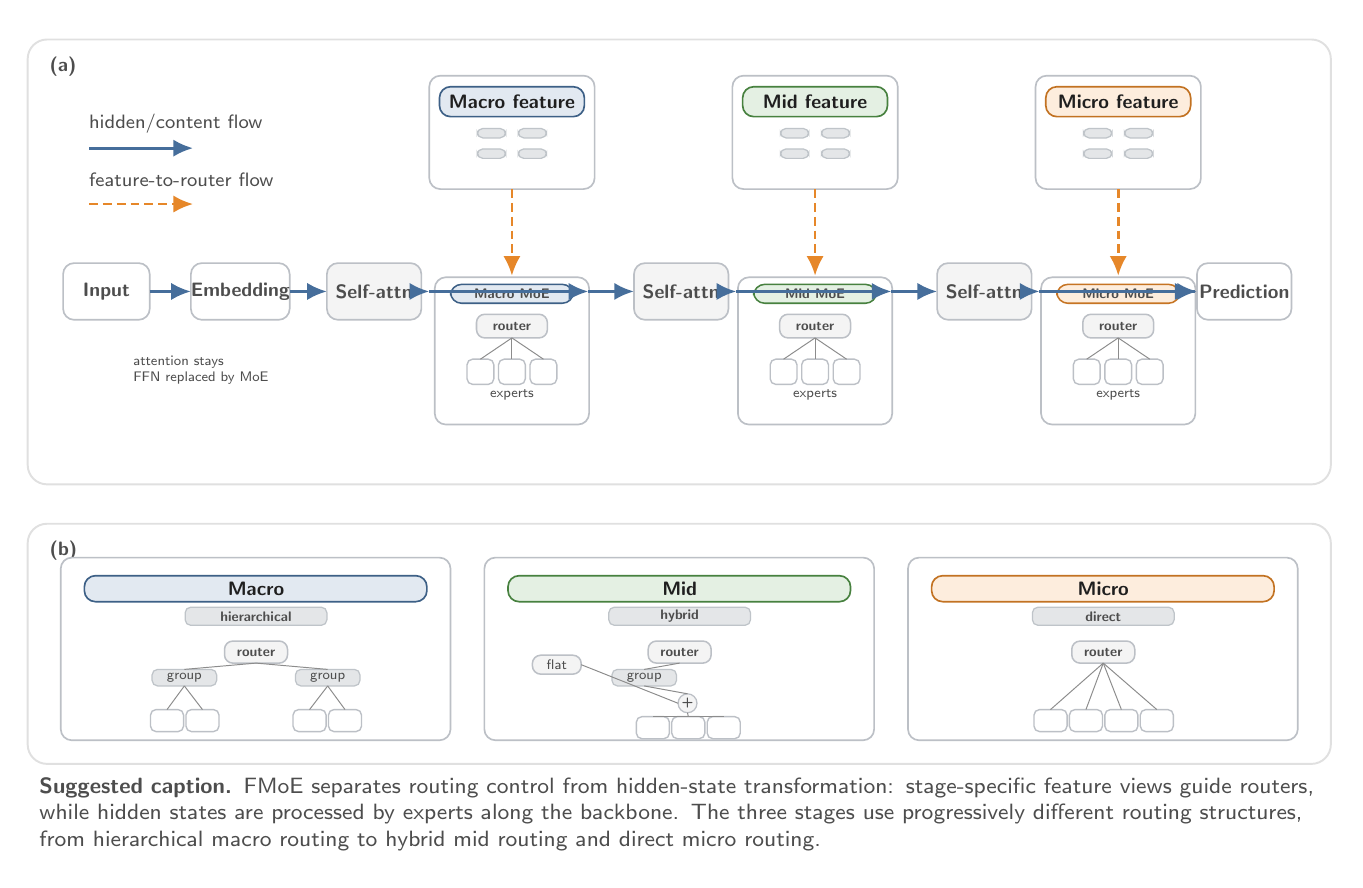
\begin{tikzpicture}[x=1cm,y=1cm]
  \path[use as bounding box] (0,-1.22) rectangle (16.6,9.35);
  \path[panelbox] (0,3.55) rectangle (16.55,9.2);
  \path[panelbox] (0,0) rectangle (16.55,3.05);
  \node[figure label, anchor=west] at (0.28,8.86) {(a)};
  \node[figure label, anchor=west] at (0.28,2.71) {(b)};

  \node[simplebox, minimum width=1.1cm, minimum height=0.72cm, font=\scriptsize\sffamily\bfseries, text=textgray] (input) at (1.0,6.0) {Input};
  \node[simplebox, minimum width=1.2cm, minimum height=0.72cm, font=\scriptsize\sffamily\bfseries, text=textgray] (embed) at (2.7,6.0) {Embedding};
  \node[attnbox, minimum width=1.2cm, minimum height=0.72cm, font=\scriptsize\sffamily\bfseries, text=textgray] (attn1) at (4.4,6.0) {Self-attn};
  \node[attnbox, minimum width=1.2cm, minimum height=0.72cm, font=\scriptsize\sffamily\bfseries, text=textgray] (attn2) at (8.3,6.0) {Self-attn};
  \node[attnbox, minimum width=1.2cm, minimum height=0.72cm, font=\scriptsize\sffamily\bfseries, text=textgray] (attn3) at (12.15,6.0) {Self-attn};
  \node[simplebox, minimum width=1.2cm, minimum height=0.72cm, font=\scriptsize\sffamily\bfseries, text=textgray] (pred) at (15.45,6.0) {Prediction};

  \begin{scope}[shift={(6.15,5.03)}]
    \path[simplebox] (-0.98,-0.72) rectangle (0.98,1.15);
    \path[draw=macroblue!80!black, fill=macroblue!16, rounded corners=4pt, line width=0.55pt] (-0.78,0.82) rectangle (0.78,1.06);
    \node[font=\tiny\sffamily\bfseries, text=textgray] at (0,0.94) {Macro MoE};
    \node[routerbox, minimum width=0.9cm, minimum height=0.3cm, font=\tiny\sffamily\bfseries, text=textgray] (r1) at (0,0.53) {router};
    \node[expertbox, minimum width=0.34cm, minimum height=0.32cm] at (-0.4,-0.05) {};
    \node[expertbox, minimum width=0.34cm, minimum height=0.32cm] at (0,-0.05) {};
    \node[expertbox, minimum width=0.34cm, minimum height=0.32cm] at (0.4,-0.05) {};
    \draw[black!45, line width=0.35pt] (r1.south) -- (-0.4,0.11);
    \draw[black!45, line width=0.35pt] (r1.south) -- (0,0.11);
    \draw[black!45, line width=0.35pt] (r1.south) -- (0.4,0.11);
    \node[font=\tiny\sffamily, text=textgray] at (0,-0.35) {experts};
  \end{scope}

  \begin{scope}[shift={(10.0,5.03)}]
    \path[simplebox] (-0.98,-0.72) rectangle (0.98,1.15);
    \path[draw=midgreen!80!black, fill=midgreen!16, rounded corners=4pt, line width=0.55pt] (-0.78,0.82) rectangle (0.78,1.06);
    \node[font=\tiny\sffamily\bfseries, text=textgray] at (0,0.94) {Mid MoE};
    \node[routerbox, minimum width=0.9cm, minimum height=0.3cm, font=\tiny\sffamily\bfseries, text=textgray] (r2) at (0,0.53) {router};
    \node[expertbox, minimum width=0.34cm, minimum height=0.32cm] at (-0.4,-0.05) {};
    \node[expertbox, minimum width=0.34cm, minimum height=0.32cm] at (0,-0.05) {};
    \node[expertbox, minimum width=0.34cm, minimum height=0.32cm] at (0.4,-0.05) {};
    \draw[black!45, line width=0.35pt] (r2.south) -- (-0.4,0.11);
    \draw[black!45, line width=0.35pt] (r2.south) -- (0,0.11);
    \draw[black!45, line width=0.35pt] (r2.south) -- (0.4,0.11);
    \node[font=\tiny\sffamily, text=textgray] at (0,-0.35) {experts};
  \end{scope}

  \begin{scope}[shift={(13.85,5.03)}]
    \path[simplebox] (-0.98,-0.72) rectangle (0.98,1.15);
    \path[draw=microorange!82!black, fill=microorange!16, rounded corners=4pt, line width=0.55pt] (-0.78,0.82) rectangle (0.78,1.06);
    \node[font=\tiny\sffamily\bfseries, text=textgray] at (0,0.94) {Micro MoE};
    \node[routerbox, minimum width=0.9cm, minimum height=0.3cm, font=\tiny\sffamily\bfseries, text=textgray] (r3) at (0,0.53) {router};
    \node[expertbox, minimum width=0.34cm, minimum height=0.32cm] at (-0.4,-0.05) {};
    \node[expertbox, minimum width=0.34cm, minimum height=0.32cm] at (0,-0.05) {};
    \node[expertbox, minimum width=0.34cm, minimum height=0.32cm] at (0.4,-0.05) {};
    \draw[black!45, line width=0.35pt] (r3.south) -- (-0.4,0.11);
    \draw[black!45, line width=0.35pt] (r3.south) -- (0,0.11);
    \draw[black!45, line width=0.35pt] (r3.south) -- (0.4,0.11);
    \node[font=\tiny\sffamily, text=textgray] at (0,-0.35) {experts};
  \end{scope}

  \draw[hiddenflow] (input.east) -- (embed.west);
  \draw[hiddenflow] (embed.east) -- (attn1.west);
  \draw[hiddenflow] (attn1.east) -- (5.1,6.0);
  \draw[hiddenflow] (5.1,6.0) -- (7.12,6.0);
  \draw[hiddenflow] (7.12,6.0) -- (attn2.west);
  \draw[hiddenflow] (attn2.east) -- (9.0,6.0);
  \draw[hiddenflow] (9.0,6.0) -- (10.97,6.0);
  \draw[hiddenflow] (10.97,6.0) -- (attn3.west);
  \draw[hiddenflow] (attn3.east) -- (12.85,6.0);
  \draw[hiddenflow] (12.85,6.0) -- (14.82,6.0);
  \draw[hiddenflow] (14.82,6.0) -- (pred.west);

  \fmoeStageCard{6.15}{8.02}{macroblue}{Macro feature}{}
  \fmoeStageCard{10.0}{8.02}{midgreen}{Mid feature}{}
  \fmoeStageCard{13.85}{8.02}{microorange}{Micro feature}{}
  \draw[featureflow] (6.15,7.3) -- (6.15,6.2);
  \draw[featureflow] (10.0,7.3) -- (10.0,6.2);
  \draw[featureflow] (13.85,7.3) -- (13.85,6.2);

  \node[legendtext, anchor=west] at (0.78,8.13) {hidden/content flow};
  \draw[hiddenflow] (0.78,7.82) -- (2.1,7.82);
  \node[legendtext, anchor=west] at (0.78,7.42) {feature-to-router flow};
  \draw[featureflow] (0.78,7.11) -- (2.1,7.11);
  \node[font=\tiny\sffamily, text=textgray, align=left] at (2.2,5.0) {attention stays\\FFN replaced by MoE};

  \begin{scope}[shift={(0.42,0.3)}]
    \foreach \x/\stagecolor/\title/\subtitle in {0.0/macroblue/Macro/hierarchical,5.38/midgreen/Mid/hybrid,10.76/microorange/Micro/direct} {
      \begin{scope}[shift={(\x,0)}]
        \path[simplebox] (0,0) rectangle (4.95,2.32);
        \path[draw=\stagecolor!80!black, fill=\stagecolor!16, rounded corners=4pt, line width=0.6pt] (0.3,1.76) rectangle (4.65,2.09);
        \node[font=\scriptsize\sffamily\bfseries, text=black!88] at (2.48,1.93) {\title};
        \path[neutralchip] (1.58,1.46) rectangle (3.38,1.69);
        \node[font=\tiny\sffamily\bfseries, text=textgray] at (2.48,1.575) {\subtitle};
      \end{scope}
    }

    % Macro wrapper: group -> expert
    \node[routerbox, minimum width=0.8cm, minimum height=0.28cm, font=\tiny\sffamily\bfseries, text=textgray] at (2.48,1.12) {router};
    \path[neutralchip] (1.16,0.69) rectangle (1.98,0.9);
    \path[neutralchip] (2.98,0.69) rectangle (3.8,0.9);
    \node[font=\tiny\sffamily, text=textgray] at (1.57,0.795) {group};
    \node[font=\tiny\sffamily, text=textgray] at (3.39,0.795) {group};
    \node[expertbox, minimum width=0.42cm, minimum height=0.28cm] at (1.35,0.25) {};
    \node[expertbox, minimum width=0.42cm, minimum height=0.28cm] at (1.8,0.25) {};
    \node[expertbox, minimum width=0.42cm, minimum height=0.28cm] at (3.16,0.25) {};
    \node[expertbox, minimum width=0.42cm, minimum height=0.28cm] at (3.61,0.25) {};
    \draw[black!45, line width=0.35pt] (2.48,0.98) -- (1.57,0.9);
    \draw[black!45, line width=0.35pt] (2.48,0.98) -- (3.39,0.9);
    \draw[black!45, line width=0.35pt] (1.57,0.69) -- (1.35,0.39);
    \draw[black!45, line width=0.35pt] (1.57,0.69) -- (1.8,0.39);
    \draw[black!45, line width=0.35pt] (3.39,0.69) -- (3.16,0.39);
    \draw[black!45, line width=0.35pt] (3.39,0.69) -- (3.61,0.39);

    % Mid wrapper: structured + flat shortcut.
    \node[routerbox, minimum width=0.8cm, minimum height=0.28cm, font=\tiny\sffamily\bfseries, text=textgray] at (7.86,1.12) {router};
    \path[neutralchip] (7.0,0.69) rectangle (7.82,0.9);
    \node[font=\tiny\sffamily, text=textgray] at (7.41,0.795) {group};
    \node[routerbox, minimum width=0.62cm, minimum height=0.24cm, font=\tiny\sffamily, text=textgray] (flat) at (6.3,0.96) {flat};
    \node[circle, draw=edgegray!95, fill=softgray, minimum size=0.24cm, line width=0.45pt] (plus) at (7.96,0.47) {};
    \node[font=\tiny\sffamily\bfseries, text=textgray] at (7.96,0.47) {+};
    \node[expertbox, minimum width=0.42cm, minimum height=0.28cm] at (7.52,0.16) {};
    \node[expertbox, minimum width=0.42cm, minimum height=0.28cm] at (7.97,0.16) {};
    \node[expertbox, minimum width=0.42cm, minimum height=0.28cm] at (8.42,0.16) {};
    \draw[black!45, line width=0.35pt] (7.86,0.98) -- (7.41,0.9);
    \draw[black!45, line width=0.35pt] (7.41,0.69) -- (plus.north);
    \draw[black!45, line width=0.35pt] (flat.east) -- (plus.west);
    \draw[black!45, line width=0.35pt] (plus.south) -- (7.97,0.3);
    \draw[black!45, line width=0.35pt] (7.97,0.3) -- (7.52,0.3);
    \draw[black!45, line width=0.35pt] (7.97,0.3) -- (8.42,0.3);

    % Micro wrapper: direct router -> expert.
    \node[routerbox, minimum width=0.8cm, minimum height=0.28cm, font=\tiny\sffamily\bfseries, text=textgray] at (13.24,1.12) {router};
    \node[expertbox, minimum width=0.42cm, minimum height=0.28cm] at (12.57,0.25) {};
    \node[expertbox, minimum width=0.42cm, minimum height=0.28cm] at (13.02,0.25) {};
    \node[expertbox, minimum width=0.42cm, minimum height=0.28cm] at (13.47,0.25) {};
    \node[expertbox, minimum width=0.42cm, minimum height=0.28cm] at (13.92,0.25) {};
    \draw[black!45, line width=0.35pt] (13.24,0.98) -- (12.57,0.39);
    \draw[black!45, line width=0.35pt] (13.24,0.98) -- (13.02,0.39);
    \draw[black!45, line width=0.35pt] (13.24,0.98) -- (13.47,0.39);
    \draw[black!45, line width=0.35pt] (13.24,0.98) -- (13.92,0.39);
  \end{scope}

  \node[anchor=north west, align=left, text width=16.22cm, font=\footnotesize\sffamily, text=textgray]
    at (0.15,-0.18) {\textbf{Suggested caption.} FMoE separates routing control from hidden-state transformation: stage-specific feature views guide routers, while hidden states are processed by experts along the backbone. The three stages use progressively different routing structures, from hierarchical macro routing to hybrid mid routing and direct micro routing.};
\end{tikzpicture}
\end{document}
